\section{Propagation d'une onde électromagnétique}
Une onde électromagnétique (OEM) est une onde qui peut se propager dans le vide
ou un milieu et qui résulte des oscillations couplées d'un champ électrique
$\v{E}$ et magnétique $\v{H}$. For a wireless link, l'information est portée par
la \emph{puissance} de l'onde électromagnétique, so everything downstream ---
lignes de transmission, adaptation d'impédance, antennes, the bilan de liaison
--- rests on knowing how $\v{E}$ and $\v{H}$ travel and how much power they
transport.

This part restricts itself to the medium in which radio and hyperfréquence links
actually live: a diélectrique parfait that is linéaire, homogène and isotrope.
Dans ce cours, on s'intéresse principalement à la propagation des ondes radio et
hyperfréquences ($\lambda > 1$ mm) pour les télécommunications. Rappel : la
fréquence $f = 1$ GHz correspond à une longueur d'onde $\lambda = 30$ cm dans
l'air.

\begin{remark}
  Si ce chapitre permet de rappeler (ou de faire découvrir pour certains) les
  fondamentaux de la propagation d'une onde électromagnétique en milieu linéaire
  homogène et isotrope, il n'est \emph{pas} au programme du contrôle. It is
  nonetheless the vocabulary --- $\eta$, $k_z$, $v_\varphi$, the vecteur de
  Poynting --- that every later chapter reuses without redefining.
\end{remark}

\begin{notation}
  In the French convention the vector operators are written
  $\overrightarrow{\mathrm{rot}}$, $\mathrm{div}$,
  $\overrightarrow{\mathrm{grad}}$; these notes write $\curl$, $\div$ and
  $\grad$ for the same three. The cross product is written $\wedge$
  throughout. Vectors are bold: $\v{E}$, $\v{H}$, $\v{k}$.\\

  Two symbols collide and must not be confused: $j$ is the imaginary unit,
  while $\v{j}(\v{r},t)$ is the current-density vector.\\

  The complex convention of the course is $e^{+j\omega t}$ for the time factor,
  so a wave travelling towards increasing $z$ carries
  $e^{j(\omega t - k_z z)}$ --- the phase spatiale enters with a \emph{minus}
  sign. Every result below inherits that sign choice.
\end{notation}

\subsection{L'onde électromagnétique dans un milieu linéaire homogène isotrope}

\begin{definition}[Milieu linéaire homogène isotrope (\textit{linear homogeneous isotropic medium}, MLHI)]
  Un milieu matériel est
  \begin{itemize}
    \item \textbf{homogène} (\textit{homogeneous}) s'il a la particularité
      d'avoir des propriétés physiques (permittivité, perméabilité,
      conductivité…) identiques en tout point de l'espace ;
    \item \textbf{isotrope} (\textit{isotropic}) s'il a la particularité
      d'avoir des propriétés physiques (permittivité, perméabilité,
      conductivité…) identiques dans toutes les directions ;
    \item \textbf{linéaire} (\textit{linear}) si la permittivité et la
      perméabilité, le caractérisant, sont indépendantes de l'amplitude du
      champ électromagnétique appliqué.
  \end{itemize}
\end{definition}

Dans le domaine des télécommunications radiofréquence, ces types de milieu sont
majoritaires (ex. : vide, air, diélectrique…) --- which is why the whole course
is written for them.

\subsubsection{Généralités sur les milieux diélectriques}

Un \textbf{milieu diélectrique} est un milieu isolant --- qui ne contient pas
des charges libres et mobiles. Les électrons présents dans un milieu
diélectrique ne peuvent pas, par définition, se déplacer sur des grandes
distances --- comme c'est le cas dans les conducteurs --- mais ont la
possibilité d'avoir des mouvements d'amplitude très petite sous l'action d'un
champ électrique $\v{E}$. Ces mouvements sont des mouvements d'oscillation
autour du noyau atomique. Le nuage électronique se déforme créant ainsi un
dipôle électrostatique (a dipole moment $\v{P}$) and hence a polarisation of the
medium. Polarisation proper --- that of the wave --- is taken up again in the
chapter on antennes.

\subsubsection{Relations constitutives des milieux diélectriques}

On appelle \textbf{relations constitutives} (\textit{constitutive relations})
d'un milieu diélectrique l'ensemble des effets du milieu sur une onde
électromagnétique. Les principales relations décrivent la susceptibilité
électrique, la permittivité diélectrique, la perméabilité magnétique et la
conductivité.

\paragraph{Susceptibilité électrique et permittivité diélectrique.}
La \textbf{susceptibilité électrique} (\textit{electric susceptibility}) $\chi$
est une grandeur caractérisant la polarisation $\v{P}$ créée par un champ
électrique $\v{E}$. L'amplitude du champ électrique utilisé est suffisamment
faible pour que la polarisation vérifie la relation suivante :
\[
  \v{P} = \varepsilon_0\,\chi\,\v{E},
  \qquad \varepsilon_0 = 8.854\,187\times 10^{-12}\ \text{F}\cdot\text{m}^{-1},
\]
où $\varepsilon_0$ est la constante diélectrique du vide. La susceptibilité
électrique $\chi$ est un nombre complexe sans dimension (le milieu, dans ce cas,
est qualifié de linéaire). Elle permet d'exprimer la permittivité diélectrique
relative par la relation :
\[
  \varepsilon_r = 1 + \Re(\chi).
\]

L'influence qu'un champ électrique $\v{E}$ a sur l'organisation des charges
électriques dans un matériau donné est définie par l'\textbf{induction
électrique} (\textit{electric displacement}) $\v{D}$. La relation entre ces
grandeurs, dans le cas d'un MLHI, est :
\[
  \v{D} = \varepsilon\,\v{E},
  \qquad\text{with}\qquad
  \varepsilon_r = \frac{\varepsilon}{\varepsilon_0},
\]
où $\varepsilon$ désigne la \textbf{permittivité} (\textit{permittivity}) sous
forme scalaire. Le vide est choisi comme milieu de référence, car il est
linéaire, homogène, isotrope avec réponse instantanée.

\begin{definition}[Angle de perte (\textit{loss angle})]
  Dans un milieu diélectrique réel, la conductivité $\sigma$ est faible mais pas
  nulle. On parle alors de \textbf{pertes diélectriques} (\textit{dielectric
  losses}). Ces pertes se traduisent en définissant une permittivité complexe
  dépendante de la fréquence ou de la pulsation de l'onde électromagnétique se
  propageant dans le milieu :
  \[
    \varepsilon(\omega) = \varepsilon'(\omega) - j\,\varepsilon''(\omega),
  \]
  et ces pertes sont souvent très faibles : la partie imaginaire est donc très
  petite devant la partie réelle, $\varepsilon''(\omega) \ll
  \varepsilon'(\omega)$. On définit alors un angle de perte $\delta$ par la
  relation :
  \[
    \tan(\delta) = \frac{\varepsilon''(\omega)}{\varepsilon'(\omega)}.
  \]
\end{definition}

Cette appellation s'explique par le fait que cet angle $\delta$ est l'angle
formé par la direction des vecteurs champ électrique $\v{E}$ et induction
électrique $\v{D}$, which are no longer collinear once $\varepsilon$ is complex.
Note the minus sign in the definition of $\varepsilon(\omega)$ --- it is what
makes a passif lossy medium sit in the fourth quadrant under the
$e^{+j\omega t}$ convention. En télécommunications, pour optimiser une liaison,
on essaiera de minimiser ces pertes.

\begin{figure}[h!]
  \centering
  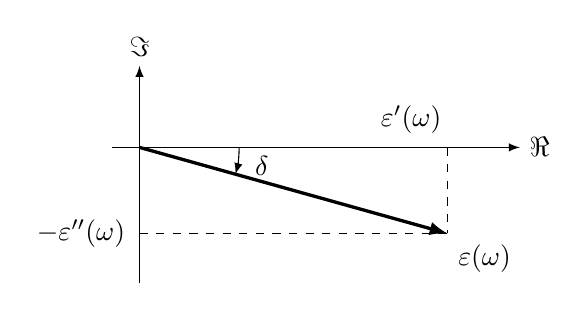
\begin{tikzpicture}[>=latex,scale=1.15]
    \draw[->] (-0.3,0) -- (4.2,0) node[right]{$\Re$};
    \draw[->] (0,-1.5) -- (0,0.9) node[above]{$\Im$};
    \draw[->,very thick] (0,0) -- (3.4,-0.95)
      node[below right]{$\varepsilon(\omega)$};
    \draw[dashed] (3.4,0) -- (3.4,-0.95);
    \draw[dashed] (0,-0.95) -- (3.4,-0.95);
    \node[above] at (3.0,0.05) {$\varepsilon'(\omega)$};
    \node[left] at (-0.05,-0.95) {$-\varepsilon''(\omega)$};
    \draw[->] (1.1,0) arc (0:-15.6:1.1);
    \node at (1.35,-0.2) {$\delta$};
  \end{tikzpicture}
  \caption*{\small The complex permittivité of a lossy diélectrique and the angle
  de perte $\delta$, with $\tan\delta = \varepsilon''/\varepsilon'$. For a
  diélectrique parfait $\varepsilon'' = 0$ and $\delta = 0$.}
\end{figure}

\begin{remark}
  En optique, on parlera plutôt d'\textbf{indice de réfraction}
  (\textit{refractive index}) du milieu, noté $n$, que de permittivité. La
  relation ci-dessous exprime le lien entre ces 2 notions :
  \[ n = \sqrt{\varepsilon_r}. \]
\end{remark}

\paragraph{Perméabilité magnétique.}
La \textbf{perméabilité magnétique} (\textit{permeability}) caractérise la
faculté d'un matériau à modifier un champ magnétique $\v{H}$, c'est-à-dire à
modifier les lignes de flux magnétique. Si le milieu a un comportement linéaire
et isotrope, le champ magnétique et l'\textbf{induction magnétique}
(\textit{magnetic induction}) $\v{B}$ sont reliés par la relation :
\[
  \v{B} = \mu\,\v{H},
  \qquad
  \mu = \mu_0\,\mu_r,
  \qquad
  \mu_0 = 4\pi\times 10^{-7}\ \text{H}\cdot\text{m}^{-1},
\]
où $\mu$ est la perméabilité magnétique du matériau (en henry par mètre, H/m)
et $\mu_r$ la perméabilité relative du matériau.

Dans l'air, le vide, les gaz, le cuivre, l'aluminium, la terre, etc.,
$\mu_r \approx 1$, ces matériaux ne pouvant alors canaliser le champ
magnétique. \textbf{Nous admettrons dans ce cours que, pour un milieu
diélectrique, $\mu_r = 1$ et que les pertes magnétiques des matériaux sont
négligeables.} Dans les milieux anisotropes, $\mu_r \ne 1$. Ces milieux
permettent la réalisation de fonctions spécifiques pour la propagation d'ondes
électromagnétiques. Nous présentons une introduction de ces milieux dans le
dernier chapitre.

\paragraph{Conductivité électrique.}
La \textbf{conductivité électrique} (\textit{conductivity}) caractérise
l'aptitude d'un matériau à laisser les charges électriques se déplacer
librement et donc permettre le passage d'un courant électrique. Elle est notée
$\sigma$ et s'exprime en $\text{S}\cdot\text{m}^{-1}$. La conductivité
s'exprime par la relation suivante, appelée aussi \textbf{loi d'Ohm locale}
(\textit{local Ohm's law}) :
\[
  \v{j} = \sigma\,\v{E},
\]
où $\v{j}$ représente la densité de courant exprimée en
$\text{A}\cdot\text{m}^{-2}$. Pour un milieu \textbf{diélectrique parfait}
(\textit{perfect dielectric}), la conductivité est nulle, $\sigma = 0$, and
therefore $\v{j} = \v{0}$.

\begin{conclusion}[Les trois relations constitutives d'un MLHI]
  \[
    \begin{array}{lll}
      \v{D} = \varepsilon\,\v{E} & \quad & \text{defines the permittivity} \\[2pt]
      \v{B} = \mu\,\v{H}         & \quad & \text{defines the permeability} \\[2pt]
      \v{j} = \sigma\,\v{E}      & \quad & \text{defines the conductivity}
    \end{array}
  \]
  with $\varepsilon = \varepsilon_0\varepsilon_r$, $\mu = \mu_0\mu_r$, and, for
  the diélectrique parfait used from here on, $\sigma = 0$ and $\mu_r = 1$.
\end{conclusion}

\subsection{Onde électromagnétique plane progressive monochromatique dans un MLHI diélectrique}

\subsubsection{Onde plane progressive}

\begin{definition}[Onde plane progressive (\textit{plane progressive wave})]
  Une onde électromagnétique est dite \textbf{plane} lorsque, pour une
  direction de propagation, les champs $\v{E}$ et $\v{H}$ conservent la même
  amplitude et même phase en tout point d'un plan orthogonal à la direction de
  propagation. La conséquence est que les variations du champ
  électromagnétique ne dépendent que de la direction de propagation. Une onde
  plane \textbf{progressive} indique que la propagation ne se fait que dans un
  sens, à partir de la source.
\end{definition}

Une onde plane est une \emph{approximation} dans le sens où c'est une
observation d'une onde dans un domaine limité de l'espace. Il suffit que les
\textbf{fronts d'onde} (\textit{wavefronts}) soient suffisamment plans et
parallèles dans le volume considéré ou en d'autres termes que l'on se trouve
suffisamment loin de la source émettant le champ électromagnétique pour pouvoir
justifier cette approximation. Dans le domaine des télécommunications radio, la
source est une antenne qui rayonne des ondes sphériques. Dans une direction
donnée et lorsqu'on est suffisamment loin, on peut considérer que localement
nous avons une onde plane.

\begin{definition}[Zones de champ rayonné par une antenne]
  Le rayonnement produit par une antenne de dimension $D$ n'est pas uniforme
  (it varies with distance). Il existe
  \begin{itemize}
    \item une \textbf{zone de champ proche} (\textit{near-field zone}),
      composée de la \textbf{zone de Rayleigh} (\textit{Rayleigh zone}) et de
      la \textbf{zone de Fresnel} (\textit{Fresnel zone}), où le front d'onde
      n'est pas plan ;
    \item la \textbf{zone de champ lointain} (\textit{far-field zone}) ou
      \textbf{zone de Fraunhofer} (\textit{Fraunhofer zone}), dont le début est
      situé à une distance
      \[ \frac{2D^2}{\lambda} \]
      de l'antenne, où $\lambda$ représente la longueur d'onde du signal émis.
  \end{itemize}
  C'est dans la zone de Fraunhofer que les ondes sont considérées localement
  planes.
\end{definition}

\begin{figure}[h!]
  \centering
  \begin{tikzpicture}[>=latex,scale=0.95]
    % aperture
    \draw[very thick] (0,-1.2) -- (0,1.2);
    \draw[<->] (-0.5,-1.2) -- (-0.5,1.2);
    \node[left] at (-0.55,0) {$D$};
    \node[below] at (-0.5,-1.3) {\small antenne};
    % beam
    \draw (0,1.2) -- (5.2,1.2) -- (8.6,2.1);
    \draw (0,-1.2) -- (5.2,-1.2) -- (8.6,-2.1);
    % zone boundaries
    \draw[dashed] (2.1,-1.55) -- (2.1,1.95);
    \draw[dashed] (5.2,-1.55) -- (5.2,1.95);
    % axis
    \draw[->] (0,0) -- (9.1,0) node[below right]{\small distance};
    % distance ticks, kept below the beam
    \node[below] at (0,-1.75) {\small $0$};
    \node[below] at (2.1,-1.7) {\small $\dfrac{D^2}{2\lambda}$};
    \node[below] at (5.2,-1.7) {\small $\dfrac{2D^2}{\lambda}$};
    % near-field bracket
    \draw[|-|] (0,2.15) -- (5.2,2.15);
    \node[above] at (2.6,2.2) {\small zone de champ proche};
    % zone labels
    \node[above,align=center] at (1.05,2.9) {\small zone de\\[-2pt]\small Rayleigh};
    \node[above,align=center] at (3.65,2.9) {\small zone de\\[-2pt]\small Fresnel};
    \node[above,align=center] at (7.2,2.9)
      {\small zone de Fraunhofer\\[-2pt]\small (champ lointain)};
  \end{tikzpicture}
  \caption*{\small Représentation des zones de champ rayonné par une antenne de
  dimension $D$. The plane-wave approximation --- and with it everything in
  this chapter --- is only legitimate beyond $2D^2/\lambda$.}
\end{figure}

Dans la zone de champ lointain, les champs $\v{E}(\v{r},t)$ et
$\v{H}(\v{r},t)$ sont perpendiculaires entre eux et perpendiculaires à la
direction de propagation. Ce type d'onde rencontrée dans les milieux
diélectriques MLHI est appelé onde \textbf{transverse électrique magnétique}
(\textit{transverse electromagnetic}, TEM).

\begin{remark}
  Il n'y aura donc \emph{pas de composante longitudinale} des champs $\v{E}$ et
  $\v{H}$ pour une onde TEM. Three vectors $\v{E}$, $\v{H}$, $\v{k}$ form a
  \textbf{trièdre direct} (\textit{right-handed trihedron}).
\end{remark}

\begin{figure}[h!]
  \centering
  \begin{tikzpicture}[>=latex,scale=1.1]
    \fill[black!7] (-1.5,-1.5) -- (0.55,-0.75) -- (0.55,1.65) -- (-1.5,0.9) -- cycle;
    \draw[black!45] (-1.5,-1.5) -- (0.55,-0.75) -- (0.55,1.65) -- (-1.5,0.9) -- cycle;
    \node[below] at (-0.5,-1.55) {\small plan d'onde};
    \draw[->,very thick] (0,0) -- (0,1.7) node[above]{$\v{E}$};
    \draw[->,very thick] (0,0) -- (-1.55,-0.58) node[left]{$\v{H}$};
    \draw[->,very thick] (0,0) -- (2.6,0)
      node[right,align=left]{$\v{k}$\\[-2pt]\small direction de propagation};
    \draw (0,0.28) -- (0.28,0.28) -- (0.28,0);
    \node[below left] at (0,0) {\small $O$};
  \end{tikzpicture}
  \caption*{\small Représentation d'une onde TEM : $\v{E} \perp \v{H} \perp
  \v{k}$, both fields lying in the wave plane, $\v{k}$ normal to it.}
\end{figure}

\subsubsection{Onde plane progressive monochromatique}

\begin{definition}[Onde monochromatique (\textit{monochromatic wave})]
  Une onde est \textbf{monochromatique} lorsque les champs $\v{E}$ et $\v{H}$,
  qui la décrivent, ne contiennent qu'une composante fréquentielle $f$ ou une
  seule pulsation $\omega = 2\pi f$. Ceci correspond donc à une onde dont la
  forme est sinusoïdale en fonction du temps et de l'espace.
\end{definition}

Dans un milieu MLHI où l'espace est matérialisé par le système de vecteur
unitaire $\v{u}(\v{u}_x,\v{u}_y,\v{u}_z)$ et $\v{r}(x,y,z)$ représentant un
point, les champs d'une \textbf{onde plane progressive monochromatique}
(\textit{plane progressive monochromatic wave}, OPPM) s'écrivent ainsi :
\[
  \begin{aligned}
    \v{E}(\v{r},t) &= \v{E}(\v{r})\cos\!\big(\omega t - \varphi(\v{r})\big) \\
    \v{H}(\v{r},t) &= \v{H}(\v{r})\cos\!\big(\omega t - \varphi(\v{r})\big)
  \end{aligned}
\]
Pour pouvoir étudier les phénomènes de propagation il est pratique de
représenter ces champs dans leur forme complexe :
\[
  \begin{aligned}
    \v{E}(\v{r},t) &= \v{E}(\v{r})\,e^{\,j(\omega t - \varphi(\v{r}))} \\
    \v{H}(\v{r},t) &= \v{H}(\v{r})\,e^{\,j(\omega t - \varphi(\v{r}))}.
  \end{aligned}
\]
Ici, $\v{E}(\v{r})$ et $\v{H}(\v{r})$ sont 2 vecteurs dont les composantes sont
transverses à la direction de propagation; which transverse directions they
pick out is the question of polarisation.\\

L'argument de l'exponentielle représente la phase des champs, and it splits in
two: le produit $\omega t$ représente la \textbf{phase temporelle}
(\textit{temporal phase}) et $\varphi(\v{r})$ la \textbf{phase spatiale}
(\textit{spatial phase}) de l'onde au vecteur position $\v{r}(x,y,z)$.

\paragraph{Variation spatiale / variation temporelle.}
Imaginons que l'on puisse arrêter le temps… On fige alors la propagation de
l'onde : on obtient la \textbf{longueur d'onde}, sur l'axe de propagation $OZ$,
en observant une période d'un signal sinusoïdal sur cet axe :
\[
  \boxed{\ \lambda = \frac{c}{f\sqrt{\varepsilon_r}}\ }
\]
où $c$ est la vitesse de la lumière dans le vide. Maintenant, imaginons un
observateur situé à l'abscisse $z$. Cet observateur va voir une variation
sinusoïdale d'amplitude de l'onde en fonction du temps. Cette variation
d'amplitude cyclique est faite sur une \textbf{période} déterminée par la
relation :
\[
  T = \frac{1}{f} = \frac{2\pi}{\omega}.
\]

\begin{figure}[h!]
  \centering
  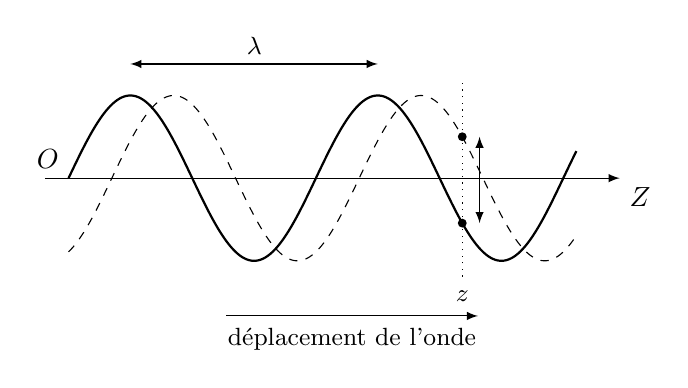
\begin{tikzpicture}[>=latex,scale=1.0]
    \draw[->] (-0.3,0) -- (7.0,0) node[below right]{$Z$};
    \node[above left] at (0,0) {$O$};
    \draw[thick,domain=0:12.9,samples=220,smooth,variable=\x]
      plot ({0.5*\x},{1.05*sin(deg(\x))});
    \draw[dashed,domain=0:12.9,samples=220,smooth,variable=\x]
      plot ({0.5*\x},{1.05*sin(deg(\x-1.1))});
    \draw[<->] (0.785,1.45) -- (3.927,1.45);
    \node[above] at (2.36,1.45) {\small $\lambda$};
    \draw[dotted] (5.0,-1.25) -- (5.0,1.25);
    \node[below] at (5.0,-1.3) {\small $z$};
    \fill (5.0,-0.571) circle (1.6pt);
    \fill (5.0,0.526) circle (1.6pt);
    \draw[<->] (5.22,-0.571) -- (5.22,0.526);
    \draw[->] (2.0,-1.75) -- (5.2,-1.75);
    \node[below] at (3.6,-1.78) {\small déplacement de l'onde};
  \end{tikzpicture}
  \caption*{\small En trait continu, l'évolution spatiale de l'onde à l'instant
  $t$ ; en pointillé, l'évolution spatiale de l'onde à l'instant
  $t + \Delta t$ avec $\Delta t < T$. The two dots are the amplitudes the
  observer at abscissa $z$ reads at the two instants: one period $\lambda$ in
  space, one period $T$ in time, the same wave.}
\end{figure}

\subsubsection{Vecteur d'onde $\v{k}$}

\begin{definition}[Vecteur d'onde (\textit{wave vector})]
  Le vecteur d'onde $\v{k}$ est un vecteur perpendiculaire au plan ou front
  d'onde et indique la direction de propagation. Sa norme correspond au
  \textbf{nombre d'onde} (\textit{wavenumber})
  \[
    \|\v{k}\| = k = \frac{2\pi}{\lambda}.
  \]
\end{definition}

De manière générale, le vecteur d'onde est défini par ses coordonnées
$\v{k}(k_x,k_y,k_z)$ exprimées dans un repère cartésien $(O,X,Y,Z)$. Dans ce
cas, on exprime la phase spatiale au point $\v{r}(x,y,z)$ :
\[
  \varphi(\v{r}) = \varphi_0 + \v{k}\cdot\v{r}
                 = \varphi_0 + \big(k_x x + k_y y + k_z z\big),
\]
où $\varphi_0$ représente la phase de l'onde à l'origine, choisie
arbitrairement car inconnue; the course sets $\varphi_0 = 0$.\\

Dans un milieu diélectrique parfait MLHI et pour une OPPM (TEM), on choisit
dans la suite du cours, par convention et simplification, une composante unique
de $\v{k}$ suivant l'axe $OZ$ :
\[
  \v{k}(0,0,k_z).
\]
Les champs $\v{E}$ et $\v{H}$ seront alors perpendiculaires entre eux et
perpendiculaires à $\v{k}$, le tout formant un trièdre direct.

\begin{conclusion}[OPPM dans un milieu MLHI se propageant selon $OZ$]
  \[
    \begin{aligned}
      \v{E}(z,t) &= \v{E}(z)\,e^{\,j(\omega t - k_z z)} \\
      \v{H}(z,t) &= \v{H}(z)\,e^{\,j(\omega t - k_z z)}
    \end{aligned}
  \]
\end{conclusion}

\subsection{Équations de Maxwell appliquées à une OPPM dans un milieu MLHI}

Les \textbf{équations de Maxwell} (\textit{Maxwell's equations}, 1864) sont des
lois fondamentales de la physique. Elles constituent la base de
l'électromagnétisme. Elles donnent ainsi un cadre mathématique précis au
concept fondamental de champ. On note $\rho$ la densité volumique de charge
électrique au point $\v{r}$ à l'instant $t$, et $\v{j}(\v{r},t)$ le vecteur
densité de courant --- attention à ne pas le confondre avec le $j$ issu des
nombres complexes.

\subsubsection{Définition des équations de Maxwell}

\begin{definition}[Maxwell--Faraday]
  L'équation de Maxwell--Faraday décrit comment la variation d'un champ
  magnétique peut induire un champ électrique. Ce courant induit est utilisé
  dans de nombreux générateurs électriques : un aimant en rotation crée un champ
  magnétique en mouvement qui génère un champ électrique dans un fil à
  proximité. Elle est définie ainsi :
  \[
    \curl \v{E} = -\frac{\del \v{B}}{\del t}
    \qquad\xrightarrow{\ \v{B} = \mu\v{H}\ }\qquad
    \curl \v{E} = -\mu\,\frac{\del \v{H}}{\del t}.
  \]
\end{definition}

\begin{definition}[Maxwell--Ampère]
  L'équation de Maxwell--Ampère énonce que les champs magnétiques peuvent être
  générés de deux manières : par les courants électriques (c'est le théorème
  d'Ampère) et par la variation d'un champ électrique (c'est l'apport de
  Maxwell sur cette loi) :
  \[
    \curl \v{H} = \v{j} + \frac{\del \v{D}}{\del t}
    \qquad\xrightarrow{\ \v{D} = \varepsilon\v{E}\ }\qquad
    \curl \v{H} = \v{j} + \varepsilon\,\frac{\del \v{E}}{\del t}.
  \]
  Dans le cas particulier d'un milieu diélectrique parfait MLHI de permittivité
  $\varepsilon$, la densité de courant est nulle, $\v{j} = \v{0}$, car il n'y a
  pas de charges électriques mobiles ou $\sigma = 0$, et on peut résumer cette
  équation par :
  \[
    \curl \v{H} = \varepsilon\,\frac{\del \v{E}}{\del t}.
  \]
\end{definition}

\begin{definition}[Maxwell--Gauss]
  Cette loi relie le flux électrique à travers n'importe quelle surface de Gauss
  fermée avec la charge électrique contenue dans le volume délimité par cette
  surface ; le champ électrique est orienté des charges positives vers les
  charges négatives :
  \[
    \div \v{D} = \rho
    \qquad\xrightarrow{\ \v{D} = \varepsilon\v{E}\ }\qquad
    \div \v{E} = \frac{\rho}{\varepsilon}.
  \]
  Dans le cas particulier d'un milieu diélectrique parfait MLHI, la densité
  volumique de charge électrique est nulle, $\rho = 0$ ; on peut alors
  simplifier l'équation par $\div \v{E} = 0$.
\end{definition}

\begin{definition}[Maxwell--Thomson]
  Le flux magnétique total à travers n'importe quelle surface de Gauss est nul :
  \[
    \div \v{B} = 0,
    \qquad\text{hence in a perfect MLHI dielectric}\qquad
    \div \v{H} = 0.
  \]
\end{definition}

\begin{remark}
  Les cas d'un diélectrique imparfait et d'un conducteur imparfait font
  apparaitre une densité de courant $\v{j}$ non nulle dans le milieu; the
  consequences for propagation --- attenuation, complex nombre d'onde --- are
  the subject of a later chapter.
\end{remark}

\begin{conclusion}[Équations de Maxwell généralisées et simplifiées]
  Les équations de Maxwell généralisées sont :
  \[
    \left\{
      \begin{aligned}
        \curl \v{E} &= -\mu\,\frac{\del \v{H}}{\del t} \\
        \curl \v{H} &= \v{j} + \varepsilon\,\frac{\del \v{E}}{\del t} \\
        \div \v{D}  &= \rho \\
        \div \v{B}  &= 0
      \end{aligned}
    \right.
  \]
  Pour une OPPM se propageant dans un milieu MLHI diélectrique parfait, de
  permittivité $\varepsilon = \varepsilon_0\varepsilon_r$ et de perméabilité
  $\mu_0$ ($\mu_r = 1$), les équations de Maxwell se simplifient ainsi :
  \[
    \left\{
      \begin{aligned}
        \curl \v{E} &= -\mu_0\,\frac{\del \v{H}}{\del t} \\
        \curl \v{H} &= \varepsilon_0\varepsilon_r\,\frac{\del \v{E}}{\del t} \\
        \div \v{E}  &= 0 \\
        \div \v{H}  &= 0
      \end{aligned}
    \right.
  \]
\end{conclusion}

\subsubsection{Opérateurs différentiels appliqués à une OPPM}

Les opérateurs vectoriels sont indépendants de la variable temporelle. On
pourra substituer les champs $\v{E}(z)$ et $\v{H}(z)$ aux champs $\v{E}(z,t)$ et
$\v{H}(z,t)$ pour simplifier l'écriture. Pour une onde monochromatique se
propageant selon $OZ$, differentiating the $e^{j\omega t}$ factor gives
\[
  \frac{\del \v{E}(z,t)}{\del t} = j\omega\,\v{E}(z)\,e^{j\omega t},
  \qquad
  \frac{\del \v{H}(z,t)}{\del t} = j\omega\,\v{H}(z)\,e^{j\omega t},
\]
and differentiating the $e^{-jk_z z}$ factor turns every $\grad$ into a
multiplication by $-j\v{k}$.

\begin{table}[h!]
  \centering
  \begin{tabular}{@{}ll@{}}
    \toprule
    \textbf{Pour $\v{E}(z)$} & \textbf{Pour $\v{H}(z)$} \\
    \midrule
    $\grad(E) = -jk\,\v{E}(z)$
      & $\grad(H) = -jk\,\v{H}(z)$ \\[4pt]
    $\div \v{E}(z) = -j\v{k}\cdot\v{E}(z) = 0$
      & $\div \v{H}(z) = -j\v{k}\cdot\v{H}(z) = 0$ \\[4pt]
    $\curl \v{E}(z) = -j\v{k}\wedge\v{E}(z)$
      & $\curl \v{H}(z) = -j\v{k}\wedge\v{H}(z)$ \\
    \bottomrule
  \end{tabular}
  \caption*{\small Opérateurs différentiels appliqués à une OPPM dans un milieu
  MLHI, avec $\v{k}(0,0,k_z)$. The two divergences vanish because $\v{k}$ is
  orthogonal to both fields --- this is exactly the TEM condition.}
\end{table}

\subsection{Équation de propagation et équation de dispersion d'une OPPM}

\subsubsection{Équation de propagation}

Start from Maxwell--Faraday in the diélectrique parfait and take the curl again:
\[
  \curl \v{E}(z,t) = -\mu_0\,\frac{\del \v{H}(z,t)}{\del t}
  \quad\Longrightarrow\quad
  \curl\big(\curl \v{E}(z,t)\big)
    = -\mu_0\,\frac{\del\big(\curl \v{H}(z,t)\big)}{\del t}
    = -\mu_0\varepsilon\,\frac{\del^2 \v{E}(z,t)}{\del t^2}.
\]
For an onde monochromatique $\del^2/\del t^2 \to (j\omega)^2 = -\omega^2$, so
\[
  \curl\big(\curl \v{E}(z,t)\big) = \omega^2\mu_0\varepsilon_0\varepsilon_r\,\v{E}(z,t).
\]
The vector identity
$\curl(\curl \v{E}) = \grad(\div \v{E}) - \Delta \v{E}$ then kills the first
term, since $\div \v{E}(z) = 0$, and leaves $-\Delta \v{E}$, with
$\Delta \v{E}(z) = \del^2\v{E}(z)/\del z^2$.

\begin{theorem}[Équation différentielle d'Helmholtz (\textit{Helmholtz differential equation})]
  \[
    \Delta\big(\v{E}(z,t)\big) + \omega^2\mu_0\varepsilon_0\varepsilon_r\,\v{E}(z,t) = 0.
  \]
  Dans le cas d'une OPPM où il n'y a aucune dépendance ou variation suivant les
  directions $OX$ et $OY$ ($\del/\del x = \del/\del y = 0$), this reduces to a
  second-order ordinary differential equation
  \[
    \frac{\del^2 \v{E}(z,t)}{\del z^2}
      + \omega^2\mu_0\varepsilon_0\varepsilon_r\,\v{E}(z,t) = 0.
  \]
\end{theorem}

\begin{prop}[Solution générale (\textit{general solution})]
  \[
    \v{E}(z,t) = \Big(
      \v{E}_+(z)\,e^{-j\omega\sqrt{\mu_0\varepsilon_0\varepsilon_r}\,z}
      + \v{E}_-(z)\,e^{+j\omega\sqrt{\mu_0\varepsilon_0\varepsilon_r}\,z}
    \Big)\,e^{j\omega t},
  \]
  où $\v{E}_+(z)$ et $\v{E}_-(z)$ sont colinéaires. De la même manière, nous
  définissons le champ magnétique :
  \[
    \v{H}(z,t) = \Big(
      \v{H}_+(z)\,e^{-j\omega\sqrt{\mu_0\varepsilon_0\varepsilon_r}\,z}
      + \v{H}_-(z)\,e^{+j\omega\sqrt{\mu_0\varepsilon_0\varepsilon_r}\,z}
    \Big)\,e^{j\omega t}.
  \]
\end{prop}

Cette solution générale indique que le champ électrique résulte de la somme
vectorielle de 2 champs électriques de même pulsation $\omega$ se déplaçant sur
le même axe de propagation, ici $OZ$, en sens opposé. On appelle, par
convention, $\v{E}_+(z)$ le \textbf{champ progressif} (\textit{progressive
field}) et $\v{E}_-(z)$ le \textbf{champ régressif} (\textit{regressive
field}). This decomposition is the seed of the whole chapter on lignes de
transmission, where the regressive wave is the one produced by a désadaptation
d'impédance.

\begin{conclusion}[Champs d'une OPPM se propageant selon $OZ$]
  Pour une OPPM associée au vecteur d'onde $\v{k}(0,0,k_z)$, se propageant dans
  un milieu MLHI diélectrique parfait, de permittivité
  $\varepsilon = \varepsilon_0\varepsilon_r$ et de perméabilité $\mu_0$, les
  champs s'écrivent :
  \[
    \begin{aligned}
      \v{E}(z,t) &= \v{E}_+(z)\,e^{\,j\omega\left(t - \sqrt{\mu_0\varepsilon_0\varepsilon_r}\,z\right)}
                  = \v{E}_+(z)\,e^{\,j(\omega t - k_z z)} \\
      \v{H}(z,t) &= \v{H}_+(z)\,e^{\,j\omega\left(t - \sqrt{\mu_0\varepsilon_0\varepsilon_r}\,z\right)}
                  = \v{H}_+(z)\,e^{\,j(\omega t - k_z z)}
    \end{aligned}
  \]
\end{conclusion}

\subsubsection{Équation de dispersion}

Avec la conclusion ci-dessus, on montre par identification --- matching the two
exponentials term by term, which is immediate --- que
\[
  k_z^{\,2} = \omega^2\mu_0\varepsilon_0\varepsilon_r.
\]

\begin{theorem}[Équation de dispersion (\textit{dispersion equation})]
  Pour une OPPM de pulsation $\omega = 2\pi f$ se propageant sur un axe $OZ$
  dans un milieu MLHI diélectrique parfait, de permittivité
  $\varepsilon = \varepsilon_0\varepsilon_r$ et de perméabilité $\mu_0$, on
  obtient l'équation de dispersion déterminant le nombre d'onde :
  \[
    \|\v{k}(0,0,k_z)\| = k_z = \frac{2\pi}{\lambda}
      = \omega\sqrt{\mu_0\varepsilon_0\varepsilon_r}.
  \]
\end{theorem}

This one relation determines everything else: it is called indifferently the
équation de dispersion or the équation de propagation, and it is what ties the
geometry of the wave ($\lambda$) to the medium ($\varepsilon_r$) and the source
($\omega$).

\subsubsection{Vitesse de propagation et longueur d'onde}

\begin{definition}[Vitesse de phase (\textit{phase velocity})]
  \[
    v_\varphi = \frac{dz}{dt} = \frac{\omega}{k}
      = \frac{1}{\sqrt{\mu_0\varepsilon_0\varepsilon_r}}
      = \frac{c}{\sqrt{\varepsilon_r}}.
  \]
  Pour une OPPM strictement monochromatique, cette vitesse est considérée comme
  la vitesse de propagation physique de l'énergie présente dans le plan d'onde.
\end{definition}

A real signal is never strictly monochromatic: une onde réelle,
quasi-monochromatique ou appelée à bande étroite (c'est le cas d'un signal
porteur d'une information à transmettre), est la superposition d'ondes planes
progressives monochromatiques (à fréquences différentes et donc de nombres
d'onde $k$ différents).

\begin{definition}[Vitesse de groupe (\textit{group velocity})]
  \[
    v_g = \frac{d\omega}{dk}.
  \]
  C'est la vitesse de propagation de l'enveloppe de l'onde réelle (ou paquet
  d'ondes). On montre qu'elle s'identifie généralement à la vitesse de
  propagation de l'énergie (ou de l'information).
\end{definition}

\begin{definition}[Milieux dispersifs et non dispersifs]
  On appellera \textbf{milieu non dispersif} (\textit{non-dispersive medium})
  les milieux où les conditions de propagation présentent l'égalité
  $v_g = v_\varphi$, c'est-à-dire où toutes les ondes se déplacent à la même
  vitesse. On appellera \textbf{milieu dispersif} (\textit{dispersive medium})
  --- fibre optique, guide d'ondes rectangulaire --- le cas où
  \[
    v_g \ne v_\varphi,
    \qquad\text{with}\qquad
    v_g < v_\varphi .
  \]
  Si un milieu diélectrique, de permittivité relative $\varepsilon_r$,
  constitue ce milieu dispersif, on peut relier la vitesse de la lumière $c$ à
  la vitesse de phase et de groupe par la relation suivante :
  \[
    \frac{c^2}{\varepsilon_r} = v_g\,v_\varphi .
  \]
\end{definition}

\begin{remark}
  The dispersive case can be stated either as $v_\varphi > c$ and $v_g < c$, or
  only as $v_g < v_\varphi$. The two are consistent with
  $c^2/\varepsilon_r = v_g v_\varphi$ when $\varepsilon_r$ is close to $1$, but
  the inequality between the two velocities is the safe one to quote: only
  $v_g$, the energy
  velocity, is bounded by $c$, and $v_\varphi$ exceeding $c$ violates nothing.
\end{remark}

Physically, au cours de la propagation, l'onde réelle --- somme d'ondes planes
sinusoïdales, sur une bande de fréquence couverte étroite mais pas nulle --- se
déforme car la vitesse de propagation dépend de la fréquence. C'est un problème
--- the limiting factor --- pour des débits de données élevés sur une longue
distance.

\begin{figure}[h!]
  \centering
  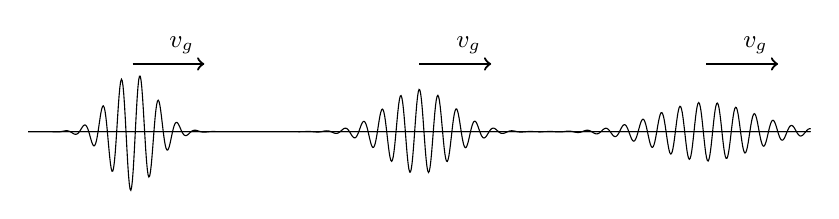
\begin{tikzpicture}
    \begin{axis}[
        width=0.95\textwidth, height=3.6cm,
        axis lines=none,
        xmin=0, xmax=12, ymin=-1.35, ymax=1.35,
        samples=1000, domain=0:12,
        clip=false,
      ]
      \addplot[black, thin] {exp(-((x-1.6)/0.5)^2)*cos(deg(22*x))};
      \addplot[black, thin] {0.72*exp(-((x-6.0)/0.72)^2)*cos(deg(22*x))};
      \addplot[black, thin] {0.50*exp(-((x-10.4)/1.05)^2)*cos(deg(22*x))};
      \draw[->,thick] (axis cs:1.6,1.15) -- (axis cs:2.7,1.15)
        node[above left]{\small $v_g$};
      \draw[->,thick] (axis cs:6.0,1.15) -- (axis cs:7.1,1.15)
        node[above left]{\small $v_g$};
      \draw[->,thick] (axis cs:10.4,1.15) -- (axis cs:11.5,1.15)
        node[above left]{\small $v_g$};
    \end{axis}
  \end{tikzpicture}
  \caption*{\small Déformation d'une onde réelle (quasi-monochromatique) dans un
  milieu dispersif: the packet travels at $v_g$ while spreading, because its
  components travel at different vitesses de phase.}
\end{figure}

\begin{definition}[Longueur d'onde]
  \[
    \lambda = \frac{2\pi}{k} = \frac{v_\varphi}{f},
    \qquad f = \frac{\omega}{2\pi}.
  \]
  Dans le cas où $\varepsilon_r = 1$, la vitesse de phase $v_\varphi = c$ et
  $\lambda = c/f$, which recovers the $\lambda = c/(f\sqrt{\varepsilon_r})$
  written earlier.
\end{definition}

\subsubsection{Impédance d'onde}

\begin{definition}[Impédance d'onde (\textit{wave impedance})]
  L'impédance d'onde $\eta$ est le rapport
  $\|\v{E}(z,t)\| \big/ \|\v{H}(z,t)\|$. Dans le cas d'une OPPM, cette
  impédance d'onde s'écrit :
  \[
    \eta = \frac{\|\v{E}_+(z)\|}{\|\v{H}_+(z)\|}
         = \frac{\omega\mu}{k}
         = \sqrt{\frac{\mu}{\varepsilon}}.
  \]
\end{definition}

Pour un milieu MLHI diélectrique avec $\mu_r = 1$ :
\[
  \eta = \sqrt{\frac{\mu_0}{\varepsilon_0\varepsilon_r}},
  \qquad\text{and for }\varepsilon_r = 1,\qquad
  \eta_0 = \sqrt{\frac{\mu_0}{\varepsilon_0}} = 120\pi\ \Omega \approx 377\ \Omega,
\]
$\eta_0$ étant l'impédance caractéristique de l'air assimilée au vide.

\begin{remark}
  One can go one step further and identify the impédance d'onde of an OPPM
  with the \textbf{impédance caractéristique du milieu de propagation}:
  \[
    Z_c = \eta = \sqrt{\frac{\mu_0}{\varepsilon_0\varepsilon_r}}.
  \]
  C'est une analogie avec la théorie des lignes de propagation autorisant un
  mode TEM --- the same $377\ \Omega$ that will reappear in the Friis bilan de
  liaison and in every antenne impedance discussion. Keep
  $377\ \Omega = 120\pi\ \Omega$ memorised; it is the single most quoted number
  of the module.
\end{remark}

\begin{example}
  In air, $\varepsilon_r \approx 1$, so $v_\varphi \approx c$ and at $f = 1$ GHz
  one gets $\lambda = 30$ cm, $k_z = 2\pi/0.30 \approx 20.9$
  $\text{rad}\cdot\text{m}^{-1}$ and $\eta \approx 377\ \Omega$.
\end{example}

\subsection{Puissance d'une OPPM dans un MLHI --- vecteur de Poynting}

\begin{definition}[Vecteur de Poynting (\textit{Poynting vector})]
  Le vecteur de Poynting, noté $\v{\Pi}$, est un vecteur dont la direction
  indique, dans un milieu MLHI, la direction de propagation d'une onde
  électromagnétique et dont l'intensité vaut la \textbf{densité de puissance}
  (\textit{power density}) véhiculée par cette onde. Le module de ce vecteur
  est donc une puissance par unité de surface ($\text{W}\cdot\text{m}^{-2}$).
  L'expression la plus générale du vecteur de Poynting est :
  \[
    \v{\Pi} = \v{E}(z,t) \wedge \v{H}(z,t).
  \]
\end{definition}

\begin{prop}[Moyenne temporelle en régime harmonique]
  Dans le cas d'une OPPM en régime harmonique, la \textbf{moyenne temporelle}
  (\textit{time average}) sur une période $T$ du vecteur de Poynting vaut :
  \[
    \langle \v{\Pi} \rangle_T
      = \tfrac{1}{2}\,\Re\!\big(\v{E}(z,t) \wedge \v{H}^{*}(z,t)\big),
  \]
  où $\v{H}^{*}(z,t)$ désigne le conjugué de $\v{H}(z,t)$.
\end{prop}

The factor $\tfrac{1}{2}$ is the usual one from averaging $\cos^2$ over a
period; the conjugation is what removes the $e^{2j\omega t}$ term and leaves a
time-independent real part.

\begin{theorem}[Puissance électromagnétique à travers une surface]
  Le flux du vecteur de Poynting à travers une surface $S$ (fermée ou non) est
  égal à la puissance véhiculée par l'onde à travers cette surface. On définit
  alors la \textbf{puissance électromagnétique} (\textit{electromagnetic power})
  de la manière suivante :
  \[
    \text{Puissance} = \iint_S \langle \v{\Pi} \rangle_T \cdot d\v{S}
      = \frac{1}{2}\,\Re\left(
          \iint_S \big(\v{E}(z,t) \wedge \v{H}^{*}(z,t)\big)\cdot d\v{S}
        \right).
  \]
\end{theorem}

Pour le cas d'une OPPM dont le champ électromagnétique est défini par les
champs établis plus haut et la définition de l'impédance d'onde $\eta$, on
écrit alors :
\[
  \v{E}(z,t) = E_+\,e^{\,j(\omega t - k_z z)}\,\v{u}_1,
  \qquad
  \v{H}(z,t) = \frac{E_+}{\eta}\,e^{\,j(\omega t - k_z z)}\,\v{u}_2,
  \qquad
  \v{u}_1 \perp \v{u}_2 \perp \v{k}_z,
\]
(rappel : pas de composante suivant $OZ$). Then
$\v{E}\wedge\v{H}^{*} = (E_+^{\,2}/\eta)\,\v{u}_1\wedge\v{u}_2$ is real and
directed along $OZ$, and

\begin{conclusion}[Puissance d'une OPPM sur une surface $S$]
  Sous condition d'onde plane sur $S$,
  \[
    \boxed{\ \text{Puissance} = \frac{E_+^{\,2}}{2\eta}\left(\iint_S d\v{S}\right)\ }
  \]
\end{conclusion}

\begin{remark}
  The two fields carry distinct unit vectors of the system $\v{u}$,
  $\v{u}_1 \perp \v{u}_2 \perp \v{k}_z$. The perpendicular pair is what makes
  the cross product non-zero and so yields the power formula above.
\end{remark}

\begin{remark}
  The form $E_+^{\,2}/2\eta$ is the field analogue of $V^2/2Z$ for an adapté
  line, and it is the quantity that the chapter on antennes integrates over a
  sphere to define puissance totale rayonnée, directivité and gain. Note that
  the power scales with the \emph{square} of the field amplitude and inversely
  with the impédance d'onde --- a medium with larger $\varepsilon_r$ has
  smaller $\eta$ and so carries more power for the same $E_+$.
\end{remark}

\subsection{La chaîne, de bout en bout}

\begin{conclusion}[What the whole part reduces to]
  Given a medium ($\varepsilon_r$, with $\mu_r = 1$, $\sigma = 0$, $\rho = 0$)
  and a source ($\omega = 2\pi f$), everything follows in one pass:
  \[
    \begin{array}{r@{\ }c@{\ }l@{\qquad}l}
      k_z &=& \omega\sqrt{\mu_0\varepsilon_0\varepsilon_r}
        & \text{dispersion equation} \\[4pt]
      v_\varphi &=& \dfrac{\omega}{k_z} = \dfrac{c}{\sqrt{\varepsilon_r}}
        & \text{phase velocity} \\[8pt]
      \lambda &=& \dfrac{2\pi}{k_z} = \dfrac{v_\varphi}{f}
                = \dfrac{c}{f\sqrt{\varepsilon_r}}
        & \text{wavelength} \\[8pt]
      \eta &=& \sqrt{\dfrac{\mu_0}{\varepsilon_0\varepsilon_r}}
             = \dfrac{\eta_0}{\sqrt{\varepsilon_r}},
             \quad \eta_0 = 120\pi \approx 377\ \Omega
        & \text{wave impedance} \\[10pt]
      \text{Puissance} &=& \dfrac{E_+^{\,2}}{2\eta}\displaystyle\iint_S d\v{S}
        & \text{power through } S
    \end{array}
  \]
  The fields themselves are $\v{E}(z,t) = \v{E}_+(z)e^{j(\omega t - k_z z)}$
  and $\v{H}(z,t) = \v{H}_+(z)e^{j(\omega t - k_z z)}$, transverse, mutually
  orthogonal, in a trièdre direct with $\v{k}$. A regressive term
  $e^{+jk_z z}$ appears only when something sends energy back --- which is
  exactly what a mismatched load on a ligne de transmission does.
\end{conclusion}
